%====================================================================================================
% Possibilities and choices
%====================================================================================================
\section{Possibilities and choices}
\subsection{Possibilities}
\subsubsection{measurement method}
Two options are available for creating the software:
\begin{enumerate}
    \item \textbf{Pre-capture of images using Vimba software (\ref{sec:Vimba})} : \newline
    In this case, the images are taken using the software supplied with the camera and then entered into the software develop with python.
    The problem is that the operator carrying out the measurement will have to switch between initialization parameters and parameters 
    for measurements on the Vimba software. For this solution, different software modes will also be required 
    \item \textbf{Image capture and analysis} :\newline
    The second solution involves automatic measurement and initialization. The operator would simply point the telescope at an 
    object and launch the software. The problem with this solution is that it would be more complex to detect a bug. In this case, 
    we'd have to come up with solutions to recognize measurement bugs as quickly as possible.
\end{enumerate}
\subsubsection{Initialization}
For initialization, two solutions are also possible :
\begin{enumerate}
    \item The first is to take several images with a exposure time equal to the measurement part. By adding up all the images, 
    the turbulence will be averaged. It will then be easy to determine the object's center of gravity and its centroid.
    \item The second option would be to considerably increase the exposure time of the image. This would be the same as the 
    previous option, but taking only 1 image would reduce memory usage and increase computing speed.
\end{enumerate}
In these 2 cases, the number of images to be used or the exposure time required to correctly average the image will need to 
be determined during the initial tests. If turbulence is not properly averaged, aberrant results may appear.
\subsubsection{Measurement}
bablablalba
\subsection{Choices}
\subsubsection{measurement method}
balbalblaba
\subsubsection{Initialization}
blalbalblalb
\subsubsection{Measurement}
bablablalba
%====================================================================================================
% Vimba software
%====================================================================================================
\section{Vimba software}\label{sec:Vimba}
blablalbal
%====================================================================================================
% Python API for Vimba
%====================================================================================================
\section{Python API for Vimba}
balbalblaba
%====================================================================================================
% The software
%====================================================================================================
\section{The software}
\subsection{Principle}
\begin{figure}[H]
    \centering
    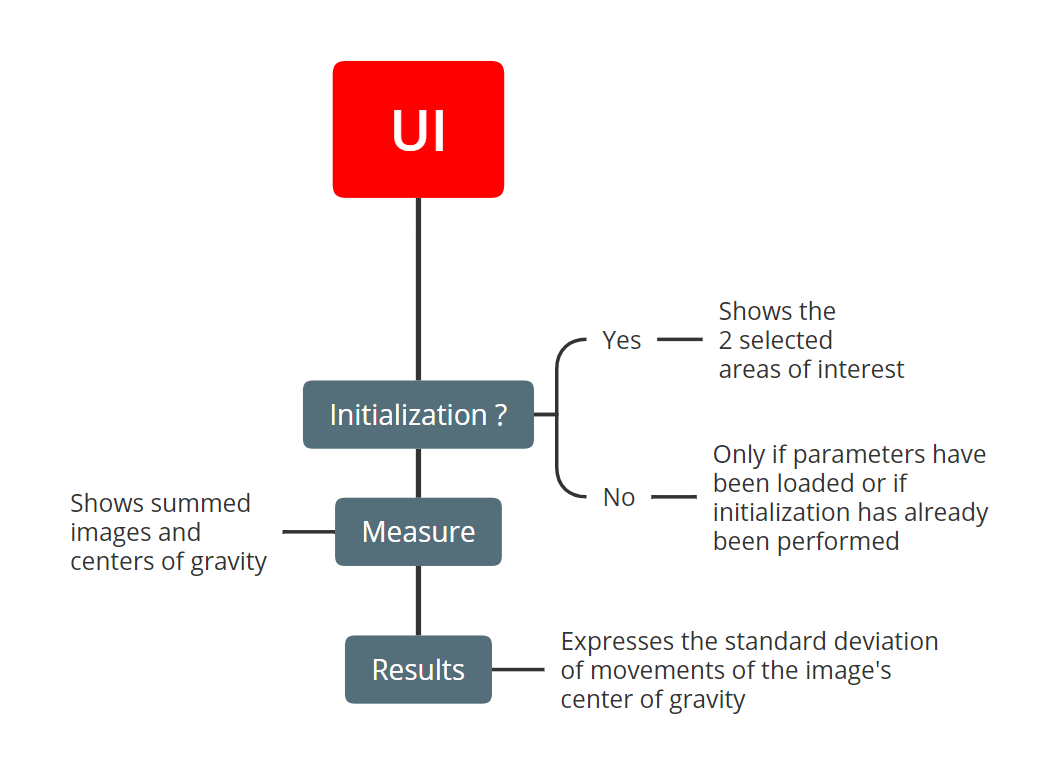
\includegraphics[scale=0.85]{assets/figures/Software/General.png}
    \caption{Software principle as seen by the user}
    \label{fig:Soft_General}
\end{figure}
\subsection{Initialisation}
\begin{figure}[H]
    \centering
    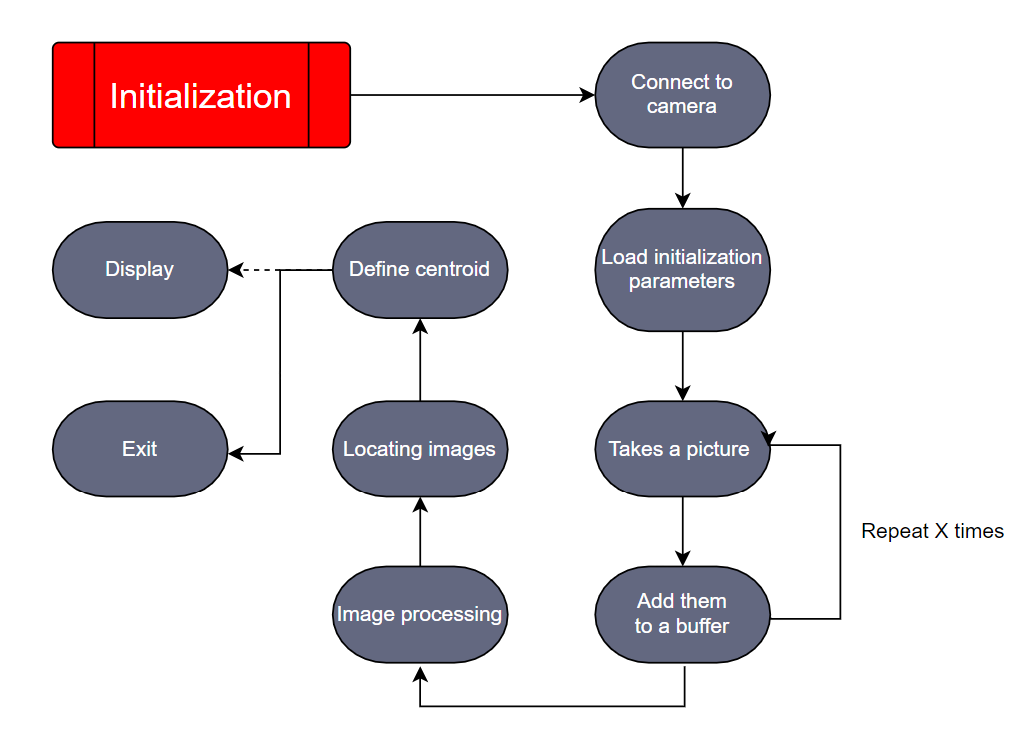
\includegraphics[scale=0.85]{assets/figures/Software/Initialization.png}
    \caption{Block diagram of the initialization function}
    \label{fig:Soft_Init}
\end{figure}
\subsection{Mesure}
blblalbalblabl
\subsection{User interface}
balbalblaba